\documentclass[10pt,a4paper]{article}

% if you use xelatex:
% \usepackage{fontspec}
% \setmainfont{Times New Roman}

\usepackage{a4wide}
\usepackage{tabularx}
\usepackage{tikz}
\usepackage{graphicx}
\usepackage[rflt]{floatflt}
\usepackage{fancyhdr}
\usepackage{amsmath}

\newcounter{num_problem}
\newcommand{\problemp}[1]{\addtocounter{num_problem}{1}{\noindent\bf Teht\"av\"a \arabic{num_problem}.} #1}
\newcommand{\problem}[1]{\problemp{#1}\medskip

}

\pagestyle{empty}
\fancyhead{}
\lhead{\sffamily Baltian tien 2009 teht\"av\"at, 7. marraskuuta, 2009}
\rhead{\sffamily Finnish}
\renewcommand{\headrulewidth}{.5pt}
\fancyfoot{}

\setlength{\headheight}{13.6pt}

\begin{document}
\rightline{\em Finnish}
\centerline{\Large \bfseries Baltian tie 2009}
\medskip
\centerline{\large \bfseries Trondheim, 7. marraskuuta, 2009}
\hspace{-1,5cm}
%\section*{Problems}
\begin{floatingfigure}[r]{.27\textwidth}
%\includegraphics[width=2cm]{/export/ghostfonts/crest.eps}  
\noindent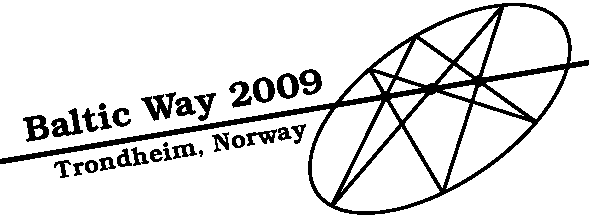
\includegraphics[width=.27\textwidth]{logo_sv}
%\caption{Using floatingfigure}
\end{floatingfigure}

\noindent Aikaa: $4\frac12$ tuntia.\smallskip

\noindent Kysymyksi\"a voi esitt\"a\"a ensimm\"aisten 30 minuutin aikana.
\vspace{4em}

\problem{
Astetta $n\geq 2$ olevalla polynomilla $p(x)$ on t\"asm\"alleen $n$ reaalista juurta, joista osa voi olla moninkertaisia. Tied\"amme, ett\"a termin $x^n$ kerroin on $1$, kaikki juuret ovat yht\"a suuria tai pienempi\"a kuin $1$ ja $p(2)=3^n$. Mit\"a arvoja voi $p(1)$ saada?
}

\problem{
Ep\"anegatiiviset kokonaisluvut $a_1, a_2, \dots ,a_{100}$ toteuttavat ep\"ayht\"al\"on
\begin{multline*}
a_1\left(a_1-1\right)\cdots \left(a_1-20\right)+a_2\left(a_2-1\right)\cdots \left(a_2-20\right)+\\ \cdots +a_{100}\left(a_{100}-1\right)\cdots \left(a_{100}-20\right) \leq 100\cdot 99\cdot 98 \cdots 79.
\end{multline*}
Osoita, ett\"a $a_1+a_2+\cdots +a_{100}\leq 9900$.
}

\problem{
Olkoon $n$ annettu positiivinen kokonaisluku. Osoita, ett\"a on mahdollista valita kertoimet $c_k\in \{-1,1\}$ ($1\leq k\leq n$) siten, ett\"a
\[
0\leq\sum_{k=1}^n c_k\cdot k^2\leq 4.
\]
}

\problem{
M\"a\"arit\"a kaikki kokonaisluvut $n>1$, joilla ep\"ayht\"al\"o
\[
x_1^2+x_2^2+\cdots +x_n^2\geq \left(x_1+x_2+\cdots +x_{n-1}\right)x_n
\]
p\"atee kaikilla reaaliluvuilla $x_1,x_2,\dots ,x_n$.
}

\problem{
Olkoon $f_0=f_1=1$ ja $f_{i+2}=f_{i+1}+f_i$ ($i\geq 0$). Ratkaise yht\"al\"o
\[
x^{2010}=f_{2009}\cdot x+f_{2008}
\] 
reaalilukujen joukossa.
}

\problem{
Olkoot $a$ ja $b$ sellaisia kokonaislukuja, ett\"a yht\"al\"oll\"a $x^3-ax^2-b=0$ on kolme kokonaislukujuurta. Osoita, ett\"a $b=dk^2$, miss\"a $d$ ja $k$ ovat kokonaislukuja ja $d$ jakaa luvun $a$.
}

\problem{
Oletetaan, ett\"a alkuluvulla $p$ ja kokonaisluvuilla $a,b,c$ seuraavat ehdot p\"atev\"at:
\[
6\mid p+1,\quad p\mid a+b+c, \quad p\mid a^4+b^4+c^4.
\]
Osoita, ett\"a $p\mid a,b,c$.
}

\problem{
M\"a\"arit\"a kaikki positiiviset kokonaisluvut $n$, joilla joukko
\[
\{n,n+1,n+2,\dots ,n+8\}
\] 
voidaan jakaa kahteen osaan  niin, ett\"a ensimm\"aisen osan alkioiden tulo on sama kuin toisen osan alkioiden tulo.
}

\problem{
M\"a\"arit\"a kaikki positiiviset kokonaisluvut $n$, joilla $2^{n+1}-n^2$ on alkuluku.
}\problem{
Olkoon $d(k)$ positiivisen kokonaisluvun $k$ positiivisten tekij\"oiden lukum\"a\"ar\"a. Osoita, ett\"a on olemassa \"a\"arett\"om\"an paljon positiivisia kokonaislukuja $M$, joita ei voida esitt\"a\"a muodossa
\[
M=\left(\frac{2\sqrt{n}}{d(n)}\right)^2
\]
mill\"a\"an positiivisella kokonaisluvulla $n$.
}

\problem{
Olkoon $M$ kolmion $ABC$ sivun $AC$ keskipiste. $K$ on piste puolisuoralla $BA$ eri puolella pistett\"a $A$ kuin $B$.  Suora $KM$ leikkaa sivun $BC$ pisteess\"a $L$. Piste $P$ on janalla $BM$ niin, ett\"a $PM$ on kulman $LPK$ puolittaja. Suora $\ell$ kulkee pisteen $A$ kautta ja on yhdensuuntainen suoran $BM$ kanssa. Osoita, ett\"a pisteen $M$ projektio suoralle $\ell$ on suoralla $PK$.
}

\problem{
Nelikulmiossa $ABCD$ on $AB\parallel CD$ ja $AB=2CD$. Suora $\ell$ on kohtisuora suoralle $CD$ ja sis\"alt\"a\"a pisteen $C$.  Ympyr\"a, jonka keskipiste on $D$ ja s\"ade $DA$ leikkaa suoran $\ell$ pisteiss\"a $P$ ja $Q$. Osoita, ett\"a $AP\bot BQ$.
}

\problem{
Piste $H$ on kolmion $ABC$ korkeusjanojen leikkauspiste ja janat $AD$, $BE$, $CF$ ovat kolmion korkeusjanat. Pisteet $I_1,I_2,I_3$ ovat kolmioiden $EHF$, $FHD$, $DHE$ sis\"a\"anpiirrettyjen ympyr\"oiden keskipisteet t\"ass\"a j\"arjestyksess\"a. Osoita, ett\"a suorat $AI_1$, $BI_2$, $CI_3$ leikkaavat yhdess\"a pisteess\"a.
}

\problem{
Mill\"a $n\geq 2$ on mahdollista l\"oyt\"a\"a $n$ pareittain ep\"ayhdenmuotoista kolmiota $A_1,A_2,\dots,A_n$ niin, ett\"a jokainen n\"aist\"a voidaan jakaa $n$ pareitttain ep\"ayhdenmuotoiseen kolmioon, joista jokainen on yhdenmuotoinen yhden kolmioista $A_1,A_2,\dots,A_n$ kanssa.
}

\problem{
Yksikk\"oneli\"o on jaettu $m$ nelikulmioon $Q_1,\ldots,Q_m$. Olkoon $S_i$ nelikulmion $Q_i$ kaikkien sivujen neli\"oiden summa jokaisella $i=1,\ldots,m$. Osoita, ett\"a
$$S_1+\ldots+S_m\geq 4.$$
}

\begin{floatingfigure}[r]{.47\textwidth}
\noindent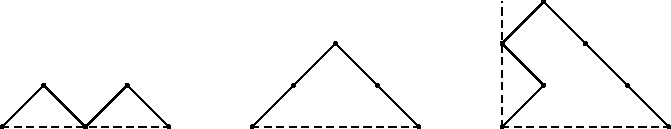
\includegraphics[width=.47\textwidth]{C2_1}
%\caption{Broken lines}
\end{floatingfigure}

\problem{
Trondheimilainen $n$-hoipertelu on k\"avely, joka l\"ahtee pisteest\"a $(0,0)$, ei leikkaa itse\"a\"an ja p\"a\"atyy pisteeseen $(2n,0)$. Lis\"aksi hoi\-per\-te\-li\-ja pysyy koor\-dinaatiston ensimm\"aisess\"a nel\-j\"an\-nek\-ses\-s\"a ja jo\-kai\-nen askel on yksi vektoreista $(1,1)$, $(1,-1)$ ja $(-1,1)$. (Kuvassa on esitetty kaikki trondheimilaiset $2$-hoipertelut.) Kuinka monta trondheimilaista $n$-hoipertelua on olemassa?
}

\problem{
Etsi suurin $n$, jolla on olemassa $n$ erisuurta kokonaislukua, joista yksik\"a\"an ei ole jaollinen yhdell\"ak\"a\"an luvuista $7$, $11$ ja $13$, mutta mink\"a tahansa kahden luvun summa on jaollinen ainakin yhdell\"a luvuista $7$, $11$ ja $13$.
}

\problem{Olkoon $n>2$ kokonaisluku. Er\"a\"ass\"a maassa on $n$ kaupunkia ja jokaisen kahden v\"aliss\"a on suora tie. Jokaisella tiell\"a on luku joukosta $\{1,2,\ldots,m\}$ (kahdella tiell\"a voi olla sama luku). Kaupungin \emph{t\"arkeysindeksi} on sinne johtavien teiden lukujen summa. Etsi pienin $m$, jolla kaikilla kaupungeilla voi olla eri t\"arkeysindeksi.
}

\problem{
Kahdeksan hengen juhlissa jokainen ihmispari joko tuntee tai ei tunne toisiaan. Jokainen ihminen tuntee t\"asm\"alleen kolme muuta. Voivatko seuraavat ehdot toteutua yht\"a aikaa:
\begin{itemize}
\item[--] miss\"a tahansa kolmen hengen joukossa on ainakin kaksi, jotka eiv\"at tunne toisiaan;
\item[--] miss\"a tahansa nelj\"an hengen joukossa on ainakin kaksi, jotka tuntevat toisensa.
\end{itemize}
}

\problem{
Tulevaisuuden Baltian Tie -kaupungissa on $16$ sairaalaa. Joka y\"o t\"asm\"alleen nelj\"a niist\"a p\"aivyst\"a\"a. Onko mahdollista j\"arjest\"a\"a aikataulu niin, ett\"a $20$ y\"on j\"alkeen mitk\"a tahansa kaksi sairaalaa olivat samassa p\"aivystysvuorossa t\"asm\"alleen kerran?
}

\end{document}
